% !TEX root = ../../../main.tex
% 来源：中学数学实验教材·第二册（几何）
% 章节：三角比与角边关系 / 解直角三角形
% 原始文件：6.tex，行 1352-1362
% 类型：tikz
% ---
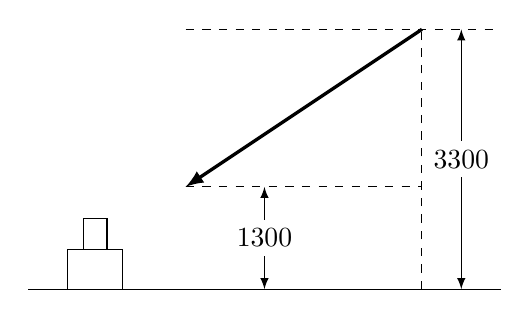
\begin{tikzpicture}[>=latex, scale=1]
\draw(-2,0)--(4,0);
\draw(-1.5,0) rectangle (-.8,.5);
\draw(-1.3,.5) rectangle (-1,.9);
\draw[dashed](0,3.3)--(4,3.3);
\draw[dashed](0,1.3)--(3,1.3);
\draw[dashed](3,0)--(3,3.3);
\draw[very thick, ->](3,3.3)--(0,1.3);
\draw[<->] (3.5,3.3)--node[fill=white]{3300}(3.5,0);
\draw[<->] (1,1.3)--node[fill=white]{1300}(1,0);
    \end{tikzpicture}
